\section{ResponseHandler Class Reference}
\label{classResponseHandler}\index{ResponseHandler@{ResponseHandler}}
{\tt \#include $<$response\_\-handler.h$>$}

Inheritance diagram for ResponseHandler:\nopagebreak
\begin{figure}[H]
\begin{center}
\leavevmode
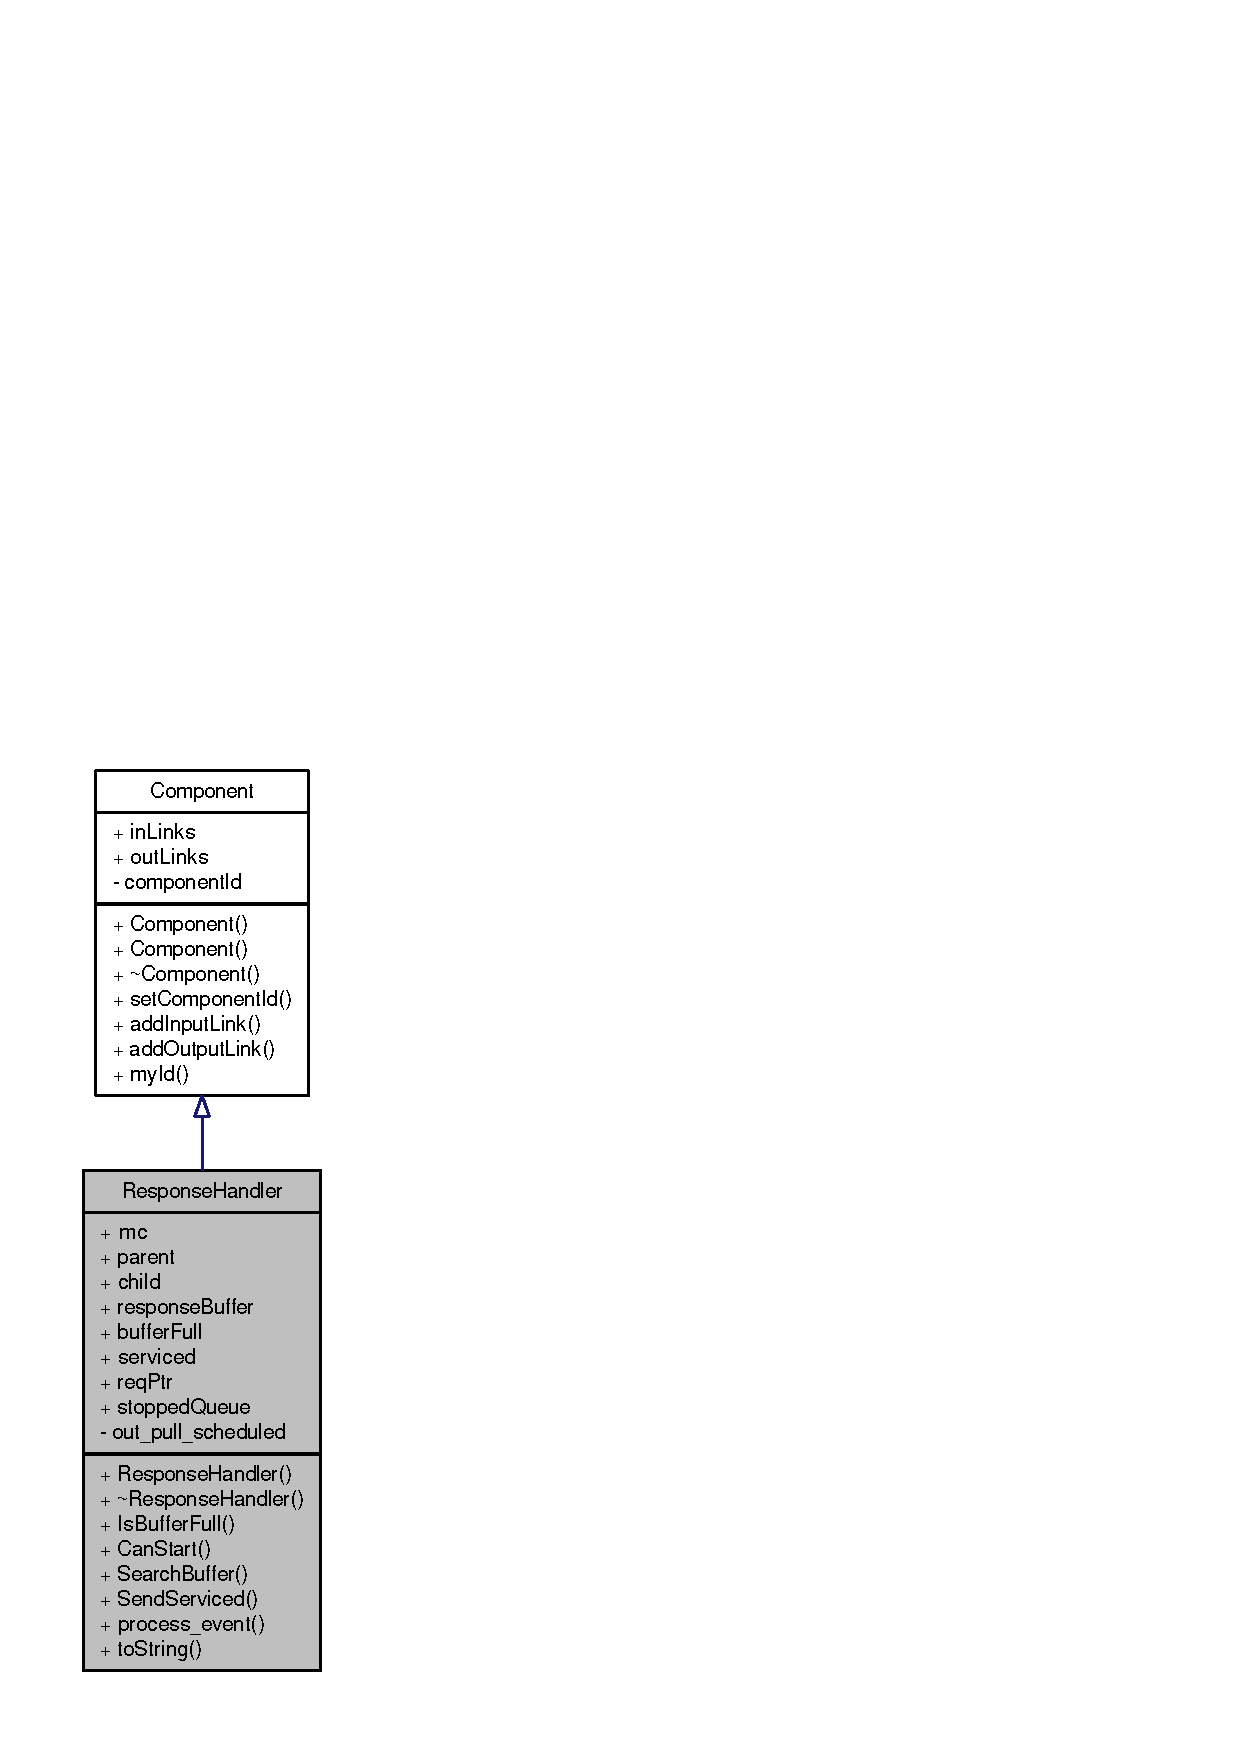
\includegraphics[height=400pt]{classResponseHandler__inherit__graph}
\end{center}
\end{figure}
Collaboration diagram for ResponseHandler:\nopagebreak
\begin{figure}[H]
\begin{center}
\leavevmode
\includegraphics[width=400pt]{classResponseHandler__coll__graph}
\end{center}
\end{figure}
\subsection*{Public Member Functions}
\begin{CompactItemize}
\item 
{\bf ResponseHandler} ()
\item 
{\bf $\sim$ResponseHandler} ()
\item 
bool {\bf IsBufferFull} ()
\item 
bool {\bf CanStart} ()
\item 
unsigned int {\bf SearchBuffer} ({\bf DRAMCmdState} $\ast$cmd)
\item 
unsigned int {\bf SendServiced} ()
\item 
void {\bf process\_\-event} ({\bf IrisEvent} $\ast$e)
\item 
std::string {\bf toString} ()
\end{CompactItemize}
\subsection*{Public Attributes}
\begin{CompactItemize}
\item 
{\bf Component} $\ast$ {\bf mc}
\item 
{\bf Component} $\ast$ {\bf parent}
\item 
{\bf Component} $\ast$ {\bf child}
\item 
vector$<$ {\bf Request} $>$ {\bf responseBuffer}
\item 
bool {\bf bufferFull}
\item 
vector$<$ bool $>$ {\bf serviced}
\item 
{\bf Component} $\ast$ {\bf reqPtr}
\item 
bool {\bf stoppedQueue}
\end{CompactItemize}
\subsection*{Private Attributes}
\begin{CompactItemize}
\item 
bool {\bf out\_\-pull\_\-scheduled}
\end{CompactItemize}


\subsection{Detailed Description}


Definition at line 47 of file response\_\-handler.h.

\subsection{Constructor \& Destructor Documentation}
\index{ResponseHandler@{ResponseHandler}!ResponseHandler@{ResponseHandler}}
\index{ResponseHandler@{ResponseHandler}!ResponseHandler@{ResponseHandler}}
\subsubsection[{ResponseHandler}]{\setlength{\rightskip}{0pt plus 5cm}ResponseHandler::ResponseHandler ()}\label{classResponseHandler_d89c619fd467111029c6ea099e9d5e74}




Definition at line 33 of file response\_\-handler.cc.

References bufferFull, RESPONSE\_\-BUFFER\_\-SIZE, responseBuffer, serviced, and stoppedQueue.\index{ResponseHandler@{ResponseHandler}!$\sim$ResponseHandler@{$\sim$ResponseHandler}}
\index{$\sim$ResponseHandler@{$\sim$ResponseHandler}!ResponseHandler@{ResponseHandler}}
\subsubsection[{$\sim$ResponseHandler}]{\setlength{\rightskip}{0pt plus 5cm}ResponseHandler::$\sim$ResponseHandler ()}\label{classResponseHandler_85af6ff6f45cc3b6fb47309f9e34729e}




Definition at line 52 of file response\_\-handler.cc.

\subsection{Member Function Documentation}
\index{ResponseHandler@{ResponseHandler}!CanStart@{CanStart}}
\index{CanStart@{CanStart}!ResponseHandler@{ResponseHandler}}
\subsubsection[{CanStart}]{\setlength{\rightskip}{0pt plus 5cm}bool ResponseHandler::CanStart ()}\label{classResponseHandler_338da4b01d1d5813e425ef3901575b86}




Definition at line 203 of file response\_\-handler.cc.

References RESPONSE\_\-BUFFER\_\-SIZE, and responseBuffer.\index{ResponseHandler@{ResponseHandler}!IsBufferFull@{IsBufferFull}}
\index{IsBufferFull@{IsBufferFull}!ResponseHandler@{ResponseHandler}}
\subsubsection[{IsBufferFull}]{\setlength{\rightskip}{0pt plus 5cm}bool ResponseHandler::IsBufferFull ()}\label{classResponseHandler_79ceeb897565c8fd54f09480f8991047}




Definition at line 189 of file response\_\-handler.cc.

References bufferFull, RESPONSE\_\-BUFFER\_\-SIZE, and responseBuffer.\index{ResponseHandler@{ResponseHandler}!process\_\-event@{process\_\-event}}
\index{process\_\-event@{process\_\-event}!ResponseHandler@{ResponseHandler}}
\subsubsection[{process\_\-event}]{\setlength{\rightskip}{0pt plus 5cm}void ResponseHandler::process\_\-event ({\bf IrisEvent} $\ast$ {\em e})}\label{classResponseHandler_da5e60fb1d62f5ca755dca334bb18f5c}




Definition at line 64 of file response\_\-handler.cc.

References Request::address, Request::arrivalTime, Request::busInsertionTime, Request::cmdType, IrisEvent::dst, IrisEvent::event\_\-data, mc, MSHR\_\-DELETE, mshrHandler, Simulator::Now(), OUT\_\-PULL\_\-EVENT, parent, NI::process\_\-event(), MSHR\_\-SA\_\-H::process\_\-event(), PUSH\_\-BUFFER, REPLY, DRAMCmdState::req, responseBuffer, Request::retireTime, Simulator::Schedule(), SearchBuffer(), SEND\_\-TO\_\-NI, SendServiced(), serviced, Request::tag, Request::threadId, and IrisEvent::type.

Referenced by NI::handle\_\-out\_\-pull\_\-event(), DataBusHandler::process\_\-event(), and BankHandler::process\_\-event().

Here is the caller graph for this function:\nopagebreak
\begin{figure}[H]
\begin{center}
\leavevmode
\includegraphics[width=420pt]{classResponseHandler_da5e60fb1d62f5ca755dca334bb18f5c_icgraph}
\end{center}
\end{figure}
\index{ResponseHandler@{ResponseHandler}!SearchBuffer@{SearchBuffer}}
\index{SearchBuffer@{SearchBuffer}!ResponseHandler@{ResponseHandler}}
\subsubsection[{SearchBuffer}]{\setlength{\rightskip}{0pt plus 5cm}unsigned int ResponseHandler::SearchBuffer ({\bf DRAMCmdState} $\ast$ {\em cmd})}\label{classResponseHandler_451d43466f59c461865559e2597040f2}




Definition at line 176 of file response\_\-handler.cc.

References DRAMCmdState::req, responseBuffer, and Request::tag.

Referenced by process\_\-event().

Here is the caller graph for this function:\nopagebreak
\begin{figure}[H]
\begin{center}
\leavevmode
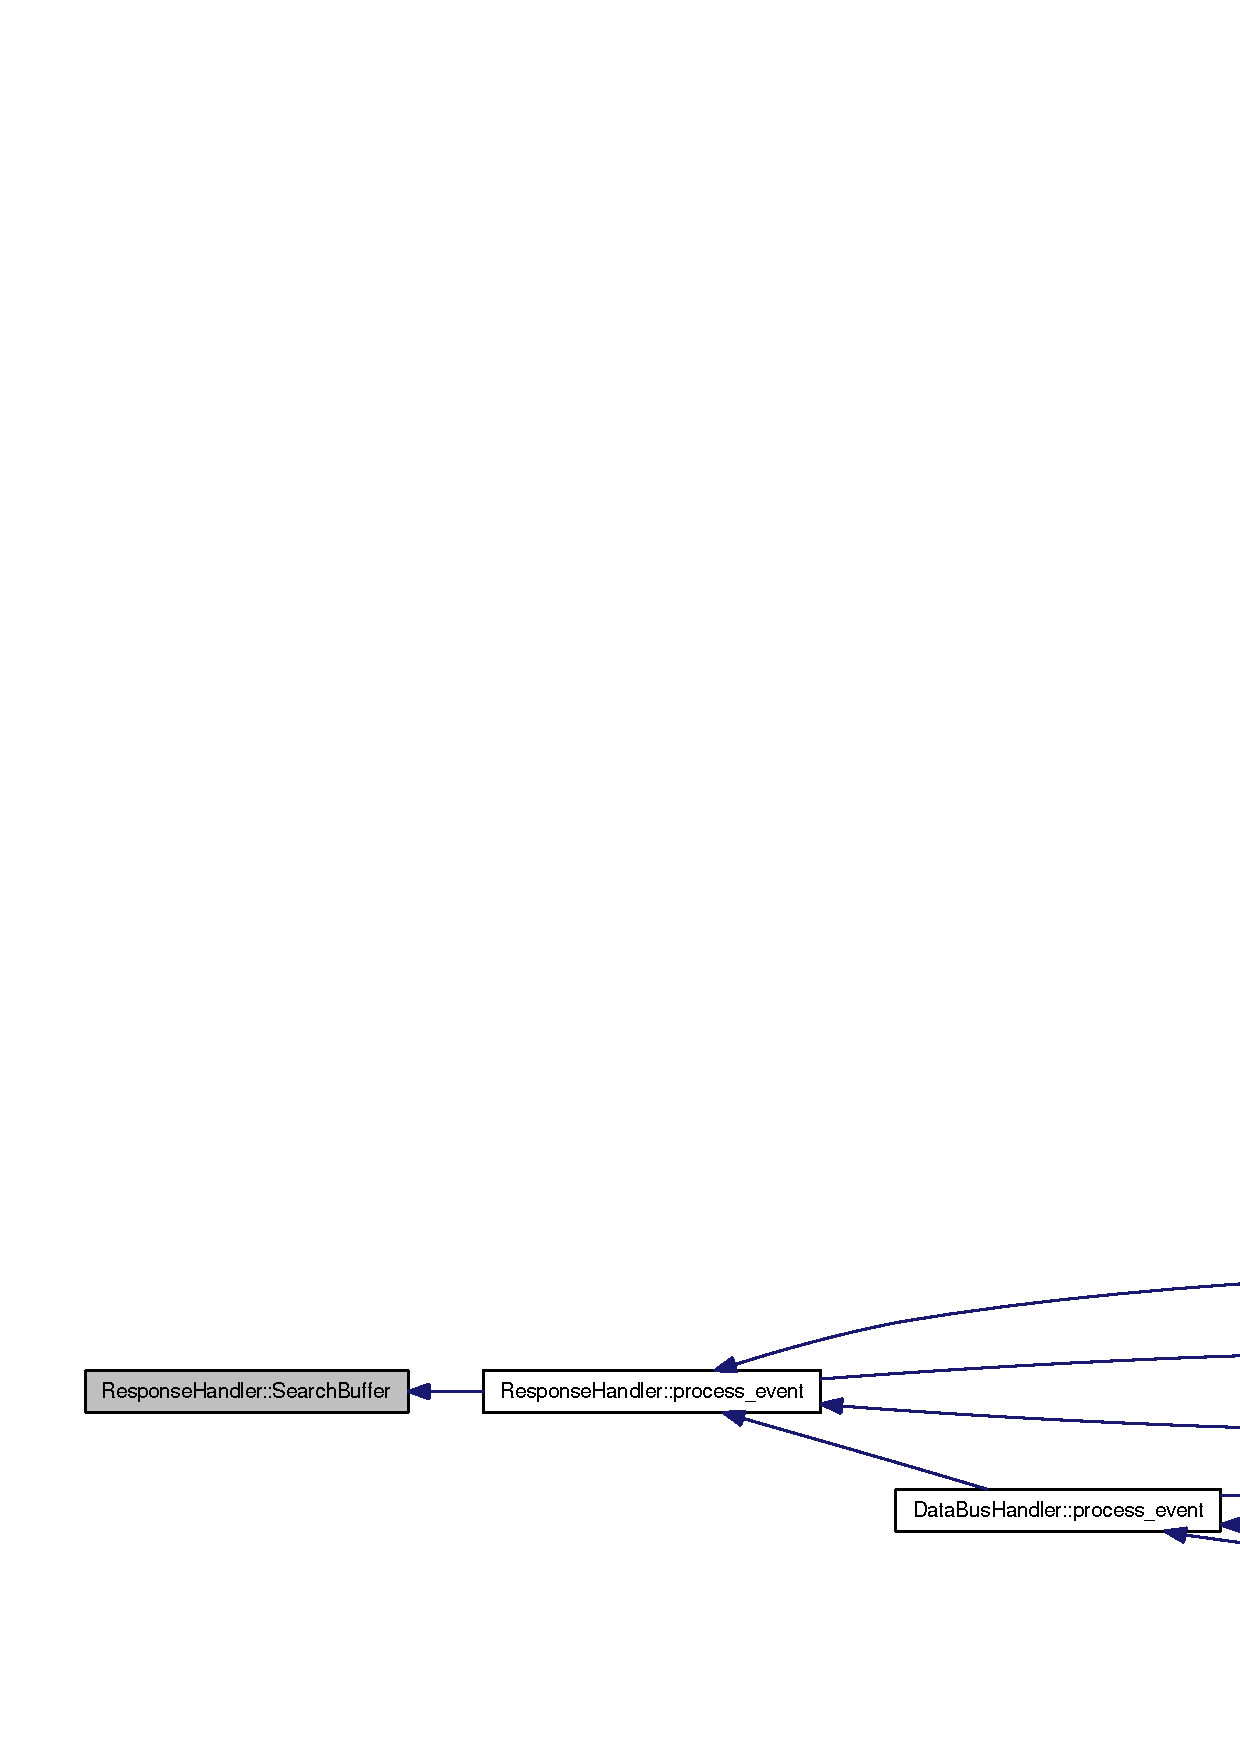
\includegraphics[width=420pt]{classResponseHandler_451d43466f59c461865559e2597040f2_icgraph}
\end{center}
\end{figure}
\index{ResponseHandler@{ResponseHandler}!SendServiced@{SendServiced}}
\index{SendServiced@{SendServiced}!ResponseHandler@{ResponseHandler}}
\subsubsection[{SendServiced}]{\setlength{\rightskip}{0pt plus 5cm}unsigned int ResponseHandler::SendServiced ()}\label{classResponseHandler_936de990ace77188310daec39b4e8d36}




Definition at line 163 of file response\_\-handler.cc.

References responseBuffer, and serviced.

Referenced by process\_\-event().

Here is the caller graph for this function:\nopagebreak
\begin{figure}[H]
\begin{center}
\leavevmode
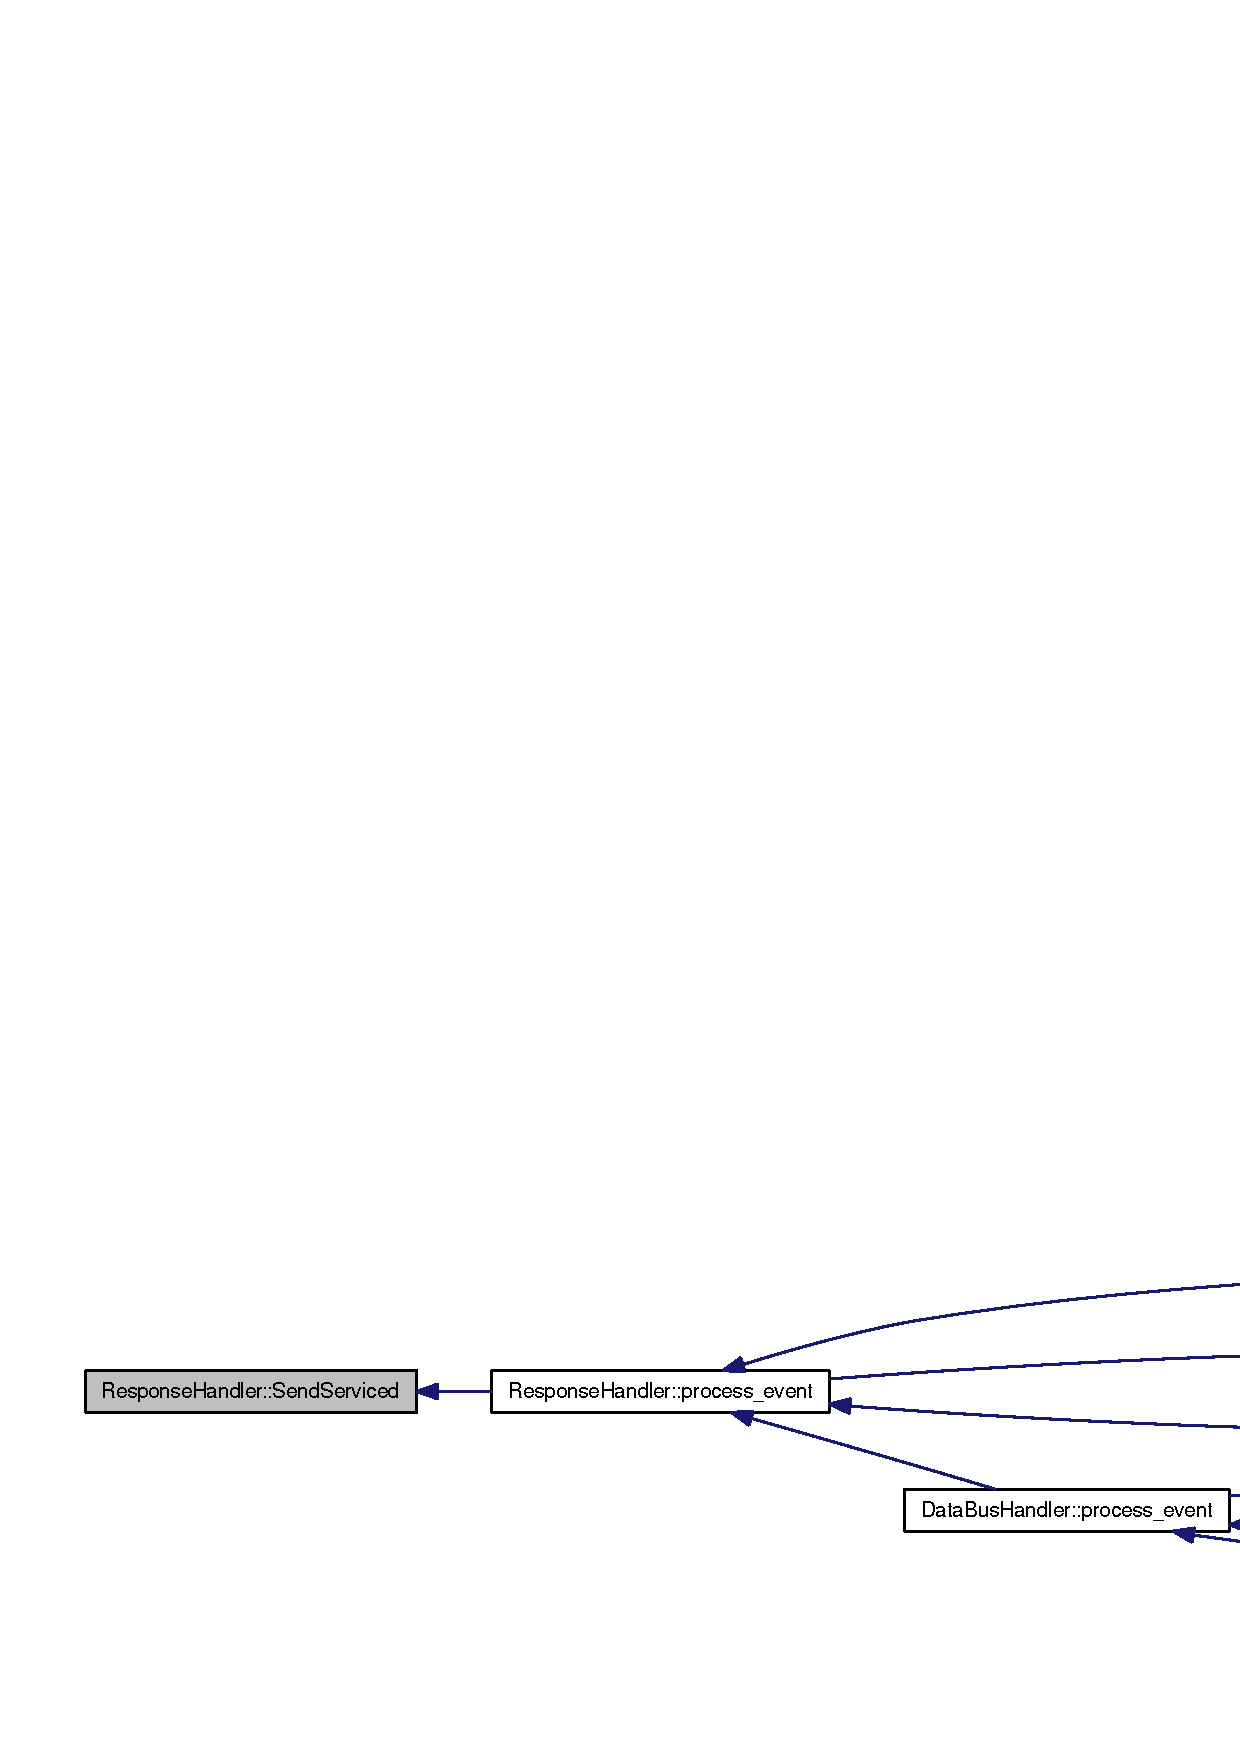
\includegraphics[width=420pt]{classResponseHandler_936de990ace77188310daec39b4e8d36_icgraph}
\end{center}
\end{figure}
\index{ResponseHandler@{ResponseHandler}!toString@{toString}}
\index{toString@{toString}!ResponseHandler@{ResponseHandler}}
\subsubsection[{toString}]{\setlength{\rightskip}{0pt plus 5cm}std::string ResponseHandler::toString ()}\label{classResponseHandler_ac99b1af9c28c04a3464ef5c60782977}




Definition at line 211 of file response\_\-handler.cc.

\subsection{Member Data Documentation}
\index{ResponseHandler@{ResponseHandler}!bufferFull@{bufferFull}}
\index{bufferFull@{bufferFull}!ResponseHandler@{ResponseHandler}}
\subsubsection[{bufferFull}]{\setlength{\rightskip}{0pt plus 5cm}bool {\bf ResponseHandler::bufferFull}}\label{classResponseHandler_205a337393bf8375b9aa5395e463011a}




Definition at line 56 of file response\_\-handler.h.

Referenced by IsBufferFull(), and ResponseHandler().\index{ResponseHandler@{ResponseHandler}!child@{child}}
\index{child@{child}!ResponseHandler@{ResponseHandler}}
\subsubsection[{child}]{\setlength{\rightskip}{0pt plus 5cm}{\bf Component}$\ast$ {\bf ResponseHandler::child}}\label{classResponseHandler_6e4e0448a89ea693f626e47d3c35214c}




Definition at line 54 of file response\_\-handler.h.

Referenced by MC::Init().\index{ResponseHandler@{ResponseHandler}!mc@{mc}}
\index{mc@{mc}!ResponseHandler@{ResponseHandler}}
\subsubsection[{mc}]{\setlength{\rightskip}{0pt plus 5cm}{\bf Component}$\ast$ {\bf ResponseHandler::mc}}\label{classResponseHandler_2181e0b35d08dcc8fc31a47ff29bcdd7}




Definition at line 52 of file response\_\-handler.h.

Referenced by MC::Init(), and process\_\-event().\index{ResponseHandler@{ResponseHandler}!out\_\-pull\_\-scheduled@{out\_\-pull\_\-scheduled}}
\index{out\_\-pull\_\-scheduled@{out\_\-pull\_\-scheduled}!ResponseHandler@{ResponseHandler}}
\subsubsection[{out\_\-pull\_\-scheduled}]{\setlength{\rightskip}{0pt plus 5cm}bool {\bf ResponseHandler::out\_\-pull\_\-scheduled}\hspace{0.3cm}{\tt  [private]}}\label{classResponseHandler_d198bc0b1d6902077d52d18f0efb3729}




Definition at line 70 of file response\_\-handler.h.\index{ResponseHandler@{ResponseHandler}!parent@{parent}}
\index{parent@{parent}!ResponseHandler@{ResponseHandler}}
\subsubsection[{parent}]{\setlength{\rightskip}{0pt plus 5cm}{\bf Component}$\ast$ {\bf ResponseHandler::parent}}\label{classResponseHandler_250c7dee041c1f3738cc53ab1dd90959}




Definition at line 53 of file response\_\-handler.h.

Referenced by MC::Init(), and process\_\-event().\index{ResponseHandler@{ResponseHandler}!reqPtr@{reqPtr}}
\index{reqPtr@{reqPtr}!ResponseHandler@{ResponseHandler}}
\subsubsection[{reqPtr}]{\setlength{\rightskip}{0pt plus 5cm}{\bf Component}$\ast$ {\bf ResponseHandler::reqPtr}}\label{classResponseHandler_b78b1fc886d81671e1353060f6cbe8c7}




Definition at line 59 of file response\_\-handler.h.

Referenced by MC::Init().\index{ResponseHandler@{ResponseHandler}!responseBuffer@{responseBuffer}}
\index{responseBuffer@{responseBuffer}!ResponseHandler@{ResponseHandler}}
\subsubsection[{responseBuffer}]{\setlength{\rightskip}{0pt plus 5cm}vector$<${\bf Request}$>$ {\bf ResponseHandler::responseBuffer}}\label{classResponseHandler_dcc85fb70179625c54862c39e6fe6fac}




Definition at line 55 of file response\_\-handler.h.

Referenced by CanStart(), IsBufferFull(), process\_\-event(), ResponseHandler(), SearchBuffer(), and SendServiced().\index{ResponseHandler@{ResponseHandler}!serviced@{serviced}}
\index{serviced@{serviced}!ResponseHandler@{ResponseHandler}}
\subsubsection[{serviced}]{\setlength{\rightskip}{0pt plus 5cm}vector$<$bool$>$ {\bf ResponseHandler::serviced}}\label{classResponseHandler_d19bac46d848111dc78b896f775a9145}




Definition at line 57 of file response\_\-handler.h.

Referenced by process\_\-event(), ResponseHandler(), and SendServiced().\index{ResponseHandler@{ResponseHandler}!stoppedQueue@{stoppedQueue}}
\index{stoppedQueue@{stoppedQueue}!ResponseHandler@{ResponseHandler}}
\subsubsection[{stoppedQueue}]{\setlength{\rightskip}{0pt plus 5cm}bool {\bf ResponseHandler::stoppedQueue}}\label{classResponseHandler_5d802125ddf42419a4d2dd1e7049bb1f}




Definition at line 60 of file response\_\-handler.h.

Referenced by ResponseHandler().

The documentation for this class was generated from the following files:\begin{CompactItemize}
\item 
{\bf response\_\-handler.h}\item 
{\bf response\_\-handler.cc}\end{CompactItemize}
